\documentclass{fkpaper}

% For marking equations using TikZ
\usetikzlibrary{tikzmark}


% Turing machine commands and stuff
\newcommand{\acceptState}{{\rm Accept}}
\newcommand{\rejectState}{{\rm Reject}}
\newcommand{\blank}{\textvisiblespace}

\newcommand{\acc}{\cmark}
\newcommand{\rej}{\cmark}

\newcommand{\lnext}{\circ}
\newcommand{\ltil}{\mathcal{U}}
\newcommand{\psc}{\mathcal{P}}

% Regular languages
\newcommand{\lreg}{\ensuremath{\ms L_{\rm reg}}}


% Command for wrapping things with きっこ brackets (requires package
% kana.sty)
%
% Named ``np'' because I couldn't think of anything better than just
% reversing ``pn''
\usepackage{kana}
\newcommand{\np}[1]{\hspace{-.55em}〔#1〕\hspace{-.55em}}

\title{DYNAMICAL SYSTEMS AND COMPUTABILITY THEORY}
\author{Forest Kobayashi and Matthew LeMay}
\affiliation{Department of Mathematics, Harvey Mudd College,
  Claremont, CA, 91711}



\begin{document}

% ----------------------------- Title ----------------------------- %



\begin{abstract}
  \textbf{Abstract goes here} Nullam eu ante vel est convallis
  dignissim. Fusce suscipit, wisi nec facilisis facilisis, est dui
  fermentum leo, quis tempor ligula erat quis odio. Nunc porta
  vulputate tellus. Nunc rutrum turpis sed pede. Sed bibendum. Aliquam
  posuere. Nunc aliquet, augue nec adipiscing interdum, lacus tellus
  malesuada massa, quis varius mi purus non odio. Pellentesque
  condimentum, magna ut suscipit hendrerit, ipsum augue ornare nulla,
  non luctus diam neque sit amet urna. Curabitur vulputate vestibulum
  lorem. Fusce sagittis, libero non molestie mollis, magna orci
  ultrices dolor, at vulputate neque nulla lacinia eros. Sed id ligula
  quis est convallis tempor. Curabitur lacinia pulvinar nibh. Nam a
  sapien.
\end{abstract}


% We propose to study the behavior of Turing Machines in the context of
% dynamical systems. A \emph{Turing Machine} (abbreviated ``TM'') is a
% model of computation involving a \emph{transition function} on a space
% of \emph{configurations}. We think of TMs as beginning with a finite
% \emph{input string} and evolving according to the rules of the
% transition function; TMs can either run forever or halt in one of the
% \emph{accepting} or \emph{rejecting} state.
% % Every TM must have a finite description;
% % however, in the course of executing a computation, we allow the TM to
% % employ an infinite ``work tape.''\footnote{This corresponds to writing
% % a computer program with finitely many characters, but allowing the
% % program to use unbounded RAM in its execution.}
% % , where each configuration represents a
% % particular combination of a \emph{state} and the contents of a
% % \emph{work
% Hence, a TM can be naturally understood as a discrete dynamical system
% with two fixed points. In this context the asymptotic behavior of TMs
% is of great interest in the field of Computability Theory; however,
% the problem has only recently begun being examined from the dynamical
% perspective. For our project we plan to examine the connection between
% these two disciplines, both in terms of how tools from abstract
% dynamical systems can help us interpret the behavior of TMs as well as
% how continuous dynamical systems can be approximated discretely to
% create analog models of computation. Particular topics of focus might
% include studying randomized approximation algorithms using the
% techniques of stability theory or investigating connections between
% the halting problem and limit cycles.

\begin{multicols}{2}
\section{Introduction}
We'll begin by introducing some of the basic vocabulary used in formal
language theory. We then discuss the layers of the \emph{Chomsky
  Hierarchy}, and how the associated models of computation for each
layer can be viewed as dynamical systems.


% We'll begin by describing some of common pieces of vocabulary used in
% computability theory.

\subsection{Strings and Alphabets}
First, we give the definitions for \emph{alphabets} and
\emph{strings}. These form the backdrop for all of our discussions of
computability theory.
\begin{definition}[Alphabet]\label{def:alphabet}
  An \emph{alphabet} is a finite set, often denoted by $\Sigma$. The
  elements of $\Sigma$ are called \emph{characters}.
\end{definition}
We make no assumptions about the characters in $\Sigma$; they will
\emph{exclusively} serve as formal symbols for use in strings.
\begin{definition}[Strings]\label{def:strings}
  Let $\Sigma$ be an alphabet. We define an operation $\cdot$ on
  $\Sigma$ as follows: Let $\sigma_1, \sigma_2 \in \Sigma$ be
  arbitrary (not necessarily distinct). Then define a \emph{new}
  symbol $\sigma_1\sigma_2$, and let
  \[
    \sigma_1 \cdot \sigma_2 = \sigma_1\sigma_2.
  \]
  Also define a special symbol $\epsilon \not\in \Sigma$ with the
  property that for all $\sigma \in \Sigma$,
  \[
    \epsilon \sigma = \sigma = \sigma \epsilon.
  \]
  Define $\Sigma^\star$ to be the collection of all formal symbols
  generated by $\Sigma \cup \set{\epsilon}$ under the operation
  $\cdot$ described above. Explicitly, if $\Sigma = \set{\sigma_1,
    \ldots, \sigma_n}$, then we have
  \begin{align*}
    \Sigma^\star
    &= \set{\epsilon,\ \np{\sigma_1},\ \ldots,\ \np{\sigma_n},\
      \np{\sigma_1 \sigma_1},\ \ldots,\ \np{\sigma_i\sigma_j},\
      \ldots} \\
    &= \bigcup_{k=0}^\infty \set{\np{\sigma_{i_1}\sigma_{i_2} \cdots
      \sigma_{i_k}} \MID \sigma_{i_j} \in \Sigma}
  \end{align*}
  Note: we are using the tortoise shell brackets〔〕just to help
  visually separate the elements. Also, when $k = 0$, we take the
  convention that $\np{} = \epsilon$. In any case, we call
  \begin{enumerate}
    \item $\Sigma^\star$ the \emph{Kleene star} of $\Sigma$,
    \item The $\cdot$ operation the \emph{concatenation operation},
      and
    \item The elements of $(\Sigma^\star, \cdot)$ \emph{strings}.
      \qedhere
  \end{enumerate}
\end{definition}
\begin{remark}
  This is the same as defining $(\Sigma^\star, \cdot)$ to be the
  \emph{free monoid} over $\Sigma$. This isn't a terribly enriching
  perspective, we just think the word ``monoid'' sounds funny so we
  wanted to say it.
\end{remark}
\begin{definition}[Length of a string]\label{def:string-length}
  Let $\Sigma$ be an alphabet, and let $\sigma \in \Sigma^\star$.
  Suppose $\sigma$ is of the form
  \[
    \sigma = \sigma_{i_1} \sigma_{i_2} \cdots \sigma_{i_k}
  \]
  where $\sigma_{i_j} \in \Sigma$ for each $j = 1, \ldots,k$. Then we
  define the \emph{length} of $\sigma$ (denoted $\abs{\sigma}$) to be
  \[
    \abs{\sigma} = k. \qedhere
  \]
\end{definition}
\begin{remark}
  Note, since $\epsilon \not\in\Sigma$, our assumption that each of
  the $\sigma_{i_j}\in \Sigma$ makes the length function well-defined.
\end{remark}
\begin{definition}[Language]\label{def:language}
  Let $\Sigma$ be an alphabet, and let $L \subseteq \Sigma^\star$.
  Then we call $L$ a \emph{language} over $\Sigma$.
\end{definition}
On their own, alphabets and strings are not very interesting. Hence
most of our questions center on \emph{languages}. One might note that
in our definition for a language, we made no requirements on $L$ other
than $L \subseteq \Sigma^\star$. Hence, $L$ could be something
extremely simple, such as
\[
  L_{\rm easy} = \set[Big]{\sigma \in \Sigma \MID \abs{\sigma}
    \equiv_2 0},
\]
or something fiendishly complex, like\footnote{Assume that we have
  some agreed-upon encoding scheme by which we can interpret strings
  in $\Sigma^\star$ as proofs.}
\[
  L_{\rm hard} = \set[Big]{\sigma \MID \text{\small $\sigma$ is a
      valid proof of Hartman–Grobman.}}
\]
We think of $L_{\rm easy}$ as having a much simpler ``structure'' when
compared to $L_{\rm hard}$. This is a byproduct of the differences in
the predicates we've use to define our sets. In the first, the rule is
very simple to state, and very simple to verify. We could imagine a
program that determines membership in $L_{\rm easy}$ simply by
scanning left-to-right and flipping a parity bit until reaching the
end of the string. Then, it would simply checks the final value of the
bit to determine whether the length of the string was even or odd. See
\cref{fig:illustration-of-process} for an illustration.
\begin{figure}[H]
  \centering
  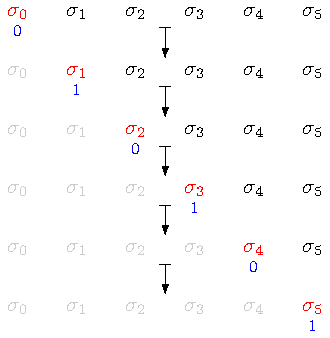
\includegraphics{figures/parity-checker.pdf}
  \caption{An illustration of the process. In each step, gray
    represents characters that've already been read, red symbols
    represent the current character, and blue symbol indicate the
    value of the parity bit. The final parity is odd, so we reject.}
  \label{fig:illustration-of-process}
\end{figure}
We note that a computer built to execute this algorithm could be very
simple: it would only need enough memory to store the program and keep
track of the parity bit, and this would be sufficient to determine
membership in $L_{\rm easy}$ for arbitrary input.

By contrast, $L_{\rm hard}$ seems a lot harder. Since the input can be
made arbitrarily long\footnote{See: this document} while still
remaining valid,\footnote{See: maybe a different document} we need to
be able to keep track of claims that are made arbitrarily far apart in
the input string. E.g., suppose we're handed something like the
following:
\begin{itemize}
  \item Axioms: $A_0$, $A_1$, \ldots, $A_n$.
  \item Desired result: $Z$.
  \item Proof:
    \begin{itemize}
      \item $1 + 1 = 2$
      % \item $2 = 2$
      \item $1 + 2 = 3$
      \item (A bunch of \np{other statements that are true but
        irrelevant} interspersed randomly with helpful ones, until
        finally)
      \item $\ldots \implies Z$.
    \end{itemize}
\end{itemize}
A priori, a verifier program has no knowledge of which claims will be
relevant later to the proof. Hence, it needs to store all of the ones
it encounters --- even silly things like $1+1 = 2$. This makes it
impossible to create an algorithm that looks exclusively at local data
to verify whether a given string $\sigma \in L_{\rm hard}$. Thus, we
would need a more sophisticated computer to execute a verifier for
$L_{\rm hard}$ than we did for $L_{\rm easy}$.


This difference is made formal by the \emph{Chomsky Hierarchy}, which
gives an ordering to languages based on the complexity of the
``computers'' needed to identify their strings.\footnote{Technically
  ``computer'' should be replaced with ``computational model,'' but
  the distinction isn't important for us today} The situation is
summarized by the following graphic:
\begin{figure}[H]
  \centering
  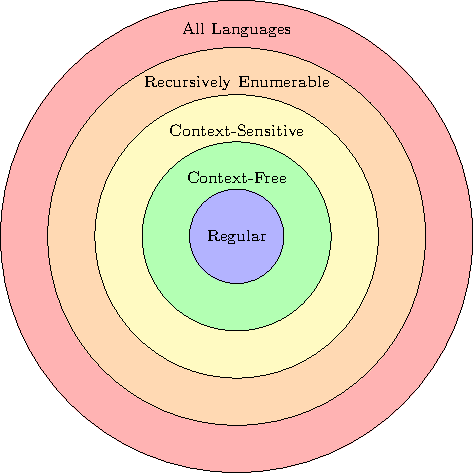
\includegraphics[scale=.8]{figures/chomsky-hierarchy.pdf}
  \caption{The Chomsky Hierarchy}
  \label{fig:chomsky-hierarchy}
\end{figure}
$L_{\rm easy}$ is a \emph{regular language}, which corresponds to one
of the simplest possible models of computation (a \emph{Deterministic
  Finite Automaton}). By contrast, $L_{\rm hard}$ requires a
\emph{Turing Machine}, one of the most powerful models of computation.
All of these can be unified into a single conceptual framework by
viewing them as \emph{dynamical systems}. The reader might consider
how as we begin with our formal definitions. But first, a quote from
Prof.\ Ran:
\begin{leftbar}
  ``There's this beautiful onion\ldots and if you cut it open, it will
  make you cry.''

  {\hfill\itshape -Prof.\ Ran, on the Chomsky Hierarchy}
\end{leftbar}
We will strive to ensure that the reader experiences only tears of
joy.


\subsection{Deterministic Finite Automata}
\emph{Deterministic finite automata} correspond to the innermost ring
of \cref{fig:chomsky-hierarchy}, the \emph{regular languages}. These
can be described formally in a number of ways; we'll choose the
following:
\begin{definition}[Regular Language]\label{def:regular-language}
  Let $\Sigma$ be an alphabet. We'll define the set of all
  \emph{regular languages over $\Sigma$} (denoted $\lreg(\Sigma)$) by
  an iterative process:
  \begin{enumerate}
    \item First, define $\varnothing$ and $\set{\epsilon}$ to be
      elements of $\lreg(\Sigma)$.
    \item Next: For all $\sigma \in \Sigma$, define $\set{\sigma}$ to
      be an element of $\lreg(\Sigma)$.
    \item Now, for all $L_0$, $L_1 \in \lreg(\Sigma)$, define
      \begin{itemize}
        \item $L_0 \cup L_1$, % {\color{red} (note, we allow only finite
          % unions)}
        \item $L_0 \cdot L_1 = \set{\ell_0 \ell_1 \MID \ell_0 \in L_0,
          \ell_1 \in L_1}$, and
        \item $L_0^\star$, $L_1^\star$
      \end{itemize}
      to be elements of $\lreg(\Sigma)$.
    \item Finally, if $L$ is yielded by a finite sequence of the
      rules above, then $L \in \lreg(\Sigma)$. \qedhere
  \end{enumerate}
\end{definition}
The idea with regular languages is that they are only slightly more
complicated than $\Sigma$ itself. Indeed, one might note the
similarity between the axioms above and those for \cref{def:strings}
(strings). We'll give a few examples of regular languages before we
introduce the associated model of computation. To that end, we'll
first introduce a shorthand that will reappear many times throughout
this paper.
\begin{definition}[Exponent notation]
  Let $\Sigma$ be an alphabet. Then for all $\sigma \in \Sigma$, we
  interpret the notation $\sigma^n$ by
  \[
    \sigma^n = \underbrace{\sigma \cdot \sigma \cdots \sigma}_{n\text{
      times}} \qedhere
  \]
\end{definition}
In light of the remark about {\color{red} m} {\color{orange} o}
{\color{yellow} n} {\color{green} o} {\color{blue} i} {\color{purple}
  d}s made earlier, this notation is actually quite reasonable.
\begin{example}\label{ex:dfa-example}
  Let $\Sigma = \set{0,1}$. Then $L$ defined by
  \[
    L = \set{0^n 1^m \MID n,m \in \NN}
  \]
  is a regular language. This follows from the fact that we can write
  $L$ as $L = \set{0}^\star \cdot \set{1}^\star$.
\end{example}
\begin{example}
  Let $\Sigma$ be an arbitrary alphabet. Then all finite sets $L
  \subseteq \Sigma$ are regular. This follows from the fact that for
  any $\sigma\in L$, if $\sigma$ decomposes as
  \[
    \sigma = \sigma_{i_1} \sigma_{i_2} \cdots \sigma_{i_k},
  \]
  Then we can state this equivalently as
  \[
    \set{\sigma} = \set{\sigma_{i_1}} \cdot \set{\sigma_{i_2}} \cdots
    \set{\sigma_{i_k}},
  \]
  from which it follows that $\set{\sigma}$ is regular. Finally, this
  gives us that
  \[
    L = \bigcup_{\sigma \in L} \set{\sigma}
  \]
  is a regular language.
\end{example}
\begin{example}
  Let $\Sigma = \set{0,1}$. Then $L$ given by $L = \set{(01)^n \MID n
    \in \NN}$ is regular.
\end{example}
As stated earlier, \emph{regular languages} are tied to
\emph{Deterministic Finite Automata}. These will lead to a more
dynamical systems-esque view of regular languages.
\begin{definition}[Deterministic Finite Automata]\label{def:dfa}
  A \emph{deterministic finite automata} is a 5-tuple
  \[
    M = (Q, F, \Sigma, \delta, q_0)
  \]
  such that the following hold:
  \begin{enumerate}
    \item $Q$, $\Sigma$, $F$ are finite sets. We choose the following
      naming conventions:
      \begin{enumerate}[label=\roman*)]
        \item $Q$ is called the \emph{set of states} for $M$,
        \item $F$ is called the set of \emph{accepting} states for
          $M$, and
        \item $\Sigma$ is called the \emph{input alphabet} for $M$;
      \end{enumerate}
    \item $\delta$ is a function $\delta : Q \times \Sigma \to Q$ (we
      call $\delta$ the \emph{transition function}), and
    \item $q_0 \in Q$ is a distinguished element that we call the
      \emph{start state}. \qedhere
  \end{enumerate}
\end{definition}
We imagine $M$ performing a computation as follows: Suppose we're
given an input string $\sigma = \sigma_{i_1} \sigma_{i_2} \ldots
\sigma_{i_k}$. $M$ initializes in the \emph{start state} $q_0$, and
reads the first character. $M$ then changes state to $q_{j_1} =
\delta(q_0, \sigma_{i_1})$, and reads the next character
$\sigma_{i_2}$. $M$ then transitions to state $q_{j_2} =
\delta(q_{j_1}, \sigma_{i_2})$, and so on. Once $M$ has exhausted the
input, it halts computation. If it halts in an \emph{accepting state}
(i.e.\ $q_{\rm final} \in F$), then we say $M$ accepts the input;
else, we say $M$ rejects it.

It's common to visualize DFAs through diagrams like the following:
\begin{figure}[H]
  \centering
  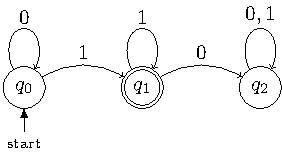
\includegraphics[scale=1.2]{figures/dfa-example.pdf}
  \caption{A DFA for \cref{ex:dfa-example}.}
\end{figure}
The convention is that circles represent states of $Q$; the arrows
represent the transitions given by $\delta(q, \sigma)$ (where $\sigma$
is the label above the arrow), and double-circled states represent
elements of $F$.

One can show that for every regular language $L$, there exists a DFA
$M_L$ such that $M_L$ accepts a string $\sigma$ iff $\sigma \in L$. We
will not give a proof today since our interests are mainly in
describing automata by dynamical systems. We now proceed in building
this up formally.

\subsection{Putting a Topology on our Strings}
We want to convert our DFAs into dynamical systems. Recall, we think
of an abstract dynamical system in terms of the following definition:
\begin{definition}[Dynamical System]
  Let $M^m$ be an $m$-manifold, and let $(T, +)$ be a monoid. Let
  $\Phi : T \times M^m \to M^m$ such that for all $x \in M^m$,
  \begin{enumerate}
    \item $\Phi(0, x) = x$, and
    \item For all $t,s \in T$, $\Phi(t + s, x) = \Phi(s, \Phi(t, x))$.
  \end{enumerate}
  Then we call $(M^m, T, \Phi)$ a \emph{dynamical system}. In
  particular, we call $M^m$ the \emph{phase space}, $t \in T$ the
  \emph{evolution parameter}, and $\Phi$ the \emph{evolution map}.
\end{definition}
To make our DFAs conform to this definition, we need to find sensible
things to call $M^m$, $T$, and $\Phi$. Let's think about what we
expect each of these to look like. The choice of evolution parameter
is easy enough; we can just think of $T$ as $\NN$ with $t=0$
corresponding to the initialization step and each $t > 0$ as
corresponding to the $n$\textsuperscript{th} step of computation.
Then, $\Phi$ will correspond to executing some step of the
computation.

The phase space is a bit trickier. For now, we'll set aside the
concerns of what it means to be an $m$-manifold and just focus on
thinking of what $M^m$ might look like as a set.

Recall that we want $M^m$ to represent all possible \emph{states} of
our system in question. In the 5-tuple formalism (\cref{def:dfa}), we
defined \emph{state} by elements of a finite set $Q$; however, this is
insufficient information to fully quantify the behavior of our DFA at
any given point of the computation --- recall that $\delta$ depends
not only on the ``state'' $q_i$, but also on the current character
being read from the input. Hence we need our dynamical version of
``state'' to include both of these pieces of information.

We might propose something like $Q \times \Sigma$ to be our state
space. But there's another problem here. Say we're given two strings
$s_0$, $s_1$:
\begin{align*}
  s_0
  &= \sigma_{i_1} \sigma_{i_2} \cdots \sigma_{i_k} \\
  s_1
  &= \sigma_{j_1} \sigma_{j_2} \cdots \sigma_{j_\ell}.
\end{align*}
Suppose now that $\sigma_{i_1} = \sigma_{j_1}$. We'll call this shared
symbol $\sigma_1$. Observe that feeding either $s_0$ or $s_1$ into
some DFA $M$ yields identical behavior in the first step:
\[
  \delta(q_0, \tikzmarknode{si1}{\sigma_{i_1}})
  = \delta(q_0, \tikzmarknode{s1}{\sigma_1})
  = \delta(q_0, \tikzmarknode{sj1}{\sigma_{j_1}})
\]
\begin{tikzpicture}[overlay, remember picture]
  \draw (si1) -- ++(0, -.25) node[coordinate, at end] (a) {};
  \draw (s1) -- ++(0, -.25) node[coordinate, at end] (b) {};
  \draw (sj1) -- ++(0, -.25) node[coordinate, at end] (c) {};
  \draw (a) -- (b) -- (c);
  \draw (b) -- ++(0,-.25) node[at end, below] {\scriptsize all equal};
\end{tikzpicture}

Hence in both cases, the machine enters some new state $q'$. But now,
suppose $\sigma_{i_2} \neq \sigma_{j_2}$, and further that $\delta(q',
\sigma_{i_2}) \neq \delta(q', \sigma_{j_2})$. Then $M$ will actually
behave differently on the two strings. Hence we see that taking our
states to be elements of $Q \times \Sigma$ also fails to give us a
full characterization of subsequent behavior.

What we really want is a way to encode the \emph{entire} unread
portion of the string into a state variable. We do exactly that with
\emph{configuartions} (note, this term is nonstandard). We will first
define \emph{unrestricted configurations}, which we'll use later in
our definition of Turing machines\footnote{We'll repeat the definition
  there when we need it, so don't worry about memorizing this one.}
We'll then define \emph{DFA configurations} as a particular restricted
subset of these unrestricted configurations.
\begin{definition}[Unrestricted Configuration]
  Given a state set $Q$ and input alphabet $\Sigma$, define the space
  of \emph{unrestricted configurations over $Q, \Sigma$} to be
  \[
    X_{\rm unrest} = Q \times \pn{\prod_{i\in \ZZ} \Sigma \cup
      \set{\epsilon}},
  \]
  where the $\prod$ is understood as a cartesian product.
\end{definition}
\begin{definition}[DFA Configuration]
  In an abuse of notation, let $\epsilon_{-\infty}^0 =
  \prod_{i=-\infty}^0$ (where the ``multiplication'' operation in
  $\prod$ is understood to be concatenation). Similarly, let
  $\epsilon_{n+1}^\infty = \prod_{i=+1}^\infty \epsilon$. Then we
  define $X_{\rm DFA}\subseteq X$ by
  \[
    X_{\rm DFA} = \set{(q, \sigma) \in X_{\rm unrest} \MID \sigma =
      \pn{\epsilon_{-\infty}^0 \cdot \np{\sigma_1 \sigma_2 \cdots
          \sigma_n} \cdot \epsilon_{n+1}^\infty}},
  \]
  where $n \in \NN$ is understood to be arbitrary, and all of the
  $\sigma_1, \ldots, \sigma_n \neq \epsilon$.
\end{definition}
Recalling that $\epsilon$ is the empty string, we see that $X_{\rm
  DFA}$ is comprised of pairs of states $q$ and finite strings
$\sigma$ over $\Sigma$ such that each string is indexed starting from
$0$. We will not need the negative indices until we discus Turing
machines.

In any case, this ``configuration space'' turns out to be the correct
choice of phase space. Woohoo! Now, all that remains is to address the
$m$-manifold condition. To that end we will first convert our
\emph{alphabets} and their \emph{strings} into sets with topological
structure. If the reader is not familiar with topology, we've included
a few definitions in the appendix --- however, we should warn that the
material below is rather technical, and hence might border on
overwhelming. We have chosen to include it because we feel it's
helpful to see how the results are all built up, since this lends
credence to later claims that the {\color{red} $p$-adic metric on
  $(\Sigma \cup \set{\epsilon})^\ZZ$ is indeed the natural choice. But
  not much will be lost to the reader who chooses just to skim, so
  feel free to do that.}


We will begin by endowing our building block sets $\Sigma \cup
\set{\epsilon}$ with a topology, and then describing how to preserve
this structure sensibly when we glue infinitely-many of them together.
\begin{definition}[Discrete Topology]
  Let $X$ be an arbitrary set. Define the \emph{discrete} topology
  $\ms T_{\rm discrete}$ on $X$ by letting every $U \subseteq X$ be an
  open set.
\end{definition}
The intuition for the \emph{discrete topology} is that it can be
realized by a metric defined by
\[
  d(x_i, x_j) =
  \begin{cases}
    c_{ij} & x_i \neq x_j \\
    0 & x_i = x_j
  \end{cases}
\]
where each $c_{ij} > 0$. In the following, we will always think of
$\Sigma \cup \set{\epsilon}$ as being endowed with the discrete
topology.
\begin{proposition}\label{prop:basis-for-strings}
  Consider $\Sigma \cup \set{\epsilon}$ with the discrete topology.
  Then the set of all singletons $\ms B = \set{\set{\varepsilon},
    \set{\sigma_1}, \set{\sigma_2}, \ldots, \set{\sigma_n}}$ forms a
  \emph{base} for $\Sigma \cup \set{\varepsilon}$.
\end{proposition}

\begin{definition}[Product Topology]
  For all $i \in I$, let $(X_i, \ms T_i)$ be a topological space. Let
  $X = \prod_{i \in I} X_i$. We define the \emph{product topology}
  $\ms T_{\rm prod}$ on $X$ as follows: For all $i \in I$, let $\pi_i
  : X \to X_i$ be the canonical projection map. Then for all open $U_i
  \subseteq X_i$, let
  \[
    \pi_i^{-1}(U_i) \in \ms T_{\rm prod}.
  \]
  We call these $\pi_i^{-1}(U_i)$ \emph{open cylinders}. Anyways: Add
  all of the sets generated by taking arbitrary unions or finite
  intersections of the open cylinders to $\ms T_{\rm prod}$. Then we
  call $\ms T_{\rm prod}$ the \emph{product} topology. \qedhere
\end{definition}
See \cref{fig:cylinder-set} for an example of an open cylinder in
$\RR^3 = \RR \times \RR^2$.

Note, the definition above abstracts on the idea that in \emph{finite}
product spaces, the projection maps $\pi_i : X \to X_i$ are
continuous, and hence preserve open sets under inverse images. This
turns out to yield a more natural topology on the product space than
we'd have if we'd defined a topology by ``products of open sets are
open in the product set.''

\begin{figure}[H]
  \centering
  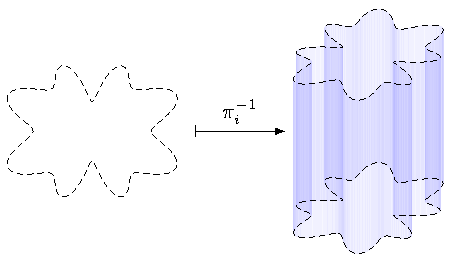
\includegraphics{figures/cylinder-set-pullback-example.pdf}
  \caption{Example partial view of a cylinder set pulled from $\RR^2$
    into $\RR^3$}
  \label{fig:cylinder-set}
\end{figure}

 % The following proposition is true for
% countable products of discrete spaces.
Product topologies can be hard to think about, so we'll try to
compartmentalize the results we want into little bite-sized steps. We
begin with a proposition that's essentially definitional, but might be
helpful as a stepping stone in building comfort. The idea is that for
a product of discrete spaces, singleton cylinders give us essentially
all we need to characterize openness.
\begin{proposition}\label{prop:singleton-cylinder}
  For all $k \in \ZZ$, let $(X_k, \ms T_k)$ be discrete topological
  spaces. Define $X = \prod_{k\in\ZZ} X_k$, and endow $X$ with the
  product topology. Fix a particular $i \in \ZZ$, and let $U_i \in\ms
  T_i$. Then for all $\sigma_j \in U_i$, $\pi_i^{-1}(\set{\sigma_j})$
  is open in $\ms T_{\rm prod}$, and $\pi_i^{-1}(U_i)$ can be written
  as
  \[
    \pi_i^{-1}(U_i) = \bigcup_{\sigma_j \in U_i}
    \pi_i^{-1}(\set{\sigma_j}). \qedhere
  \]
\end{proposition}
\begin{sproof}
  Note that since $X_i$ has the discrete topology, for all $\sigma_j
  \in U_j$, $\set{\sigma_j} \in \ms T_j$. Thus
  $\pi_i^{-1}(\set{\sigma_j})$ is an open cylinder, and hence open (by
  definition of $\ms T_{\rm prod}$). The union part follows
  immediately by definition; let's write it out explicitly. The
  important part is highlighted in {\color{blue} blue}. By definition,
  \begin{align*}
    \pi_i^{-1}(U_i)
    &= \pn{\prod_{k = -\infty}^{i-1} X_k} \times {\color{blue} U_i}
      \times \pn{\prod_{k=i+1}^\infty X_k} \\
    &= \pn{\prod_{k = -\infty}^{i-1} X_k} \times {\color{blue}
      \bigcup_{\sigma_j \in U_i} \set{\sigma_j}} \times
      \pn{\prod_{k=i+1}^\infty X_k} \\
    &= {\color{blue} \bigcup_{\sigma_j \in U_i}} \pn{\prod_{k =
      -\infty}^{i-1} X_k} \times {\color{blue} \set{\sigma_j}} \times
      \pn{\prod_{k=i+1}^\infty X_k} \\
    &= {\color{blue} \bigcup_{\sigma_j \in U_i}}
      \pi_i^{-1}({\color{blue} \set{\sigma_j}}),
  \end{align*}
  as desired. \qedhere
\end{sproof}
Now, we observe that it's not generally true that the product of
discrete spaces is discrete under the product topology. Indeed, we
actually only get discrete-like behavior when we look at subsets of a
particular form. We'll prove this over a series of claims in the
below. First, we prove a general result for product spaces.
\begin{proposition}\label{prop:openness-in-products}
  For all $k \in \ZZ$, let $(X_k, \ms T_k)$ be topological spaces. Let
  $X = \prod_{k \in \ZZ} X_k$. Then $U \subseteq X$ is open iff $U$ is
  of the form $\prod_{k \in \ZZ} U_k$, where only finitely-many of the
  $U_k \neq X_k$.
\end{proposition}
\begin{sproof}
  Since $U$ is open, then by definition of $\ms T_{\rm prod}$, $U$ can
  be expressed as an arbitrary union of \np{intersections of open
    cylinders} (in the following, let $V_{j_\ell} \subseteq X_{j_\ell}$):
  \[
    A = \bigcup_{i \in I} \bigcap_{j_\ell = j_1}^{j_{k_i}}
    \pi_{j_\ell}^{-1}(V_{j_\ell}).
  \]
  The extra $\ell$ subscript on the $j_\ell$ index is just meant to encode
  that for different $i$'s, we could be picking different families of
  $U_j$'s to use in the intersection.\footnote{E.g., for $i = 1$, we
    might pick $j \in \set{1, 3, 5, \ldots, 21}$, whereas for $i = 2$,
    we might have $j \in \set{2, 3, 5, 7, 13, \ldots, 23}$, or
    something.} For each $i \in I$, let
  \[
    j_{i, {\rm max}} = \max_{j_\ell = j_1, \ldots, j_{k_i}} \set{j_\ell}.
  \]
  And similarly for $j_{i, {\rm min}}$. Then observe that for all $i$,
  for all $k > j_{i, {\rm max}}$ or $k < j_{i, {\rm min}}$, we have
  \[
    \pi_{k} \pn{\bigcap_{j_\ell = j_1}^{j_{k_i}}
      \pi_{j_\ell}^{-1}(V_{j_\ell})} = X_{k}.
  \]
  Hence, it's only possible for $U_k \neq X_k$ for $j_{i, {\rm
      min}}\leq n \leq j_{i, {\rm max}}$, which represents
  finitely-many of the $U_n$.
\end{sproof}
\begin{proposition}\label{prop:clopen-discrete}
  With all variables quantified as above, if each of the $X_k$'s have
  the discrete topology, then one can replace ``open'' with
  ``clopen.''
\end{proposition}
Before proving this, we should first remind ourselves of how set
complement behaves over cartesian products. Given sets $A,B$, and
subsets $S \subseteq A$, $T \subseteq B$, then we have
\[
  (S \times T)^c = (S^c \times T^c) \cup (S^c \times T) \cup (S
  \times T^c),
\]
and \textbf{\emph{NOT}}
\[
  (S \times T)^c = S^c \times T^c. \quad {\color{red} \xmark \text{
      no!}}
\]
In particular, when $T = B$, we have
\[
  (S \times B)^c = S^c \times B. \qedhere
\]
\begin{sproof}
  In light of the note above, it suffices to show that if each of the
  $X_k$'s are given the discrete topology, then the complement of an
  open cylinder $\pi_i^{-1}(U_i)$ is an open cylinder. This follows
  directly from applying \cref{prop:singleton-cylinder} to $U_i^c$.
\end{sproof}
We have one final proposition, which the reader should think of in
terms of the context of $X_{\rm unrest}$. Like all claims involving
the product topology, the statement looks technical, but it's saying
something very simple: Namely, open balls in $X$ are collections of
sequences that share a common portion around the
$0$\textsuperscript{th} character.

\textbf{Note:} For the sake of making things fit on one line, we'll
use the notation
\[
  X_{-\infty}^{k_1} = \prod_{i=-\infty}^{k_1}X_i
  \qquad\text{and}\qquad
  X_{k_2+1}^{\infty} = \prod_{i=k_2+1}^{\infty}X_i
\]
in the following. We'll also interpret the somewhat-incomprehensible
notation
\[
  \bigcup_{x_i \in X_i} \pn{\prod_{i = k_1}^{k_2} \set{x_i}}
\]
quite liberally as ``all possible strings of characters that could
appear between index $k_1$ and $k_2$ inclusive.''
\begin{proposition}\label{prop:prefix-basis}
  For all $k \in \ZZ$, let $(X_k, \ms T_k)$ be discrete topological
  spaces. Define $X = \prod_{k\in\ZZ} X_k$.%  In the below, fo each $k
  % \in \ZZ^{\geq 0}$ (nonnegative integers) and for each $i \in
  % \set{-k, \ldots, k}$, we'll use $x_i$ to denote an arbitrary element
  % of $X_i$.
  Then the collection $\ms B$ given by
  \[
    \ms B = \bigcup_{\substack{k_1, k_2 \in \ZZ \\ k_1 \leq 0 \leq k_2}}
    \bigcup_{x_i \in X_i} X_{-\infty}^{k_1-1} \times
    % \set{x_{k_1}} \times \cdots \times \set{x_{k_2}}
    \pn{\prod_{i = k_1}^{k_2} \set{x_i}}
    \times X_{k_2+1}^\infty
  \]
  defines a topological base for $\ms T_{\rm prod}$.
\end{proposition}
Again, since we've had to make multiple notational compromises here,
we'll take the opportunity to clarify what a prototypical element of
$\ms B$ looks like. It's a collection of \emph{all} bi-directional
sequences that are identical in the {\color{blue} blue} portion of
$\cdots \sigma_{k_1-1} {\color{blue} \sigma_{k_1} \cdots \sigma_{k_2}}
\sigma_{k_2+1} \cdots$, where $k_1 \leq 0 \leq k_2$.

The unions we use to define $\ms B$ range over all possible choices of
endpoints $k_1 \leq 0 \leq k_2$, and for fixed $k_1$, $k_2$, over all
possible values for the blue portion itself.
\begin{sproof}
  We are using the definition of a base given in \cref{def:base}.
  First, note that
  \[
    X = \bigcup_{B \in \ms B} B,
  \]
  hence $\ms B$ satisfies the covering axiom for a base. We want to
  show it satisfies the second. Let $B_1, B_2 \in \ms B$ be
  arbitrarily chosen. Write these as
  \begin{align*}
    B_1
    &= X_{-\infty}^{\ell_1-1}\times \set{x_{1,\ell_1} } \times
      \cdots \times \set{x_{1,\ell_2}} \times X_{\ell_2+1}^\infty \\
    B_2
    &= X_{-\infty}^{m_1-1}\times \set{x_{1,m_1} } \times \cdots \times
      \set{x_{1,m_2}} \times X_{m_2+1}^\infty
  \end{align*}
  We have two cases.
  \begin{enumerate}
    \item Suppose there exists $k \in \set{\max\set{\ell_1, m_1},
      \ldots, \min\set{\ell_2, m_2}}$ such that $x_{1,k} \neq
      x_{2,k}$. Then $B_1 \cap B_2 = \varnothing$. Thus in this case,
      the ``intersection stuff'' axiom for a base is satisfied
      vacuously. \cmark
    \item Suppose that no such $k$ exists. Let $k_1 = \min\set{\ell_1,
      m_1}$ and $k_2 = \max\set{\ell_2, m_2}$ (note, this is the
      opposite of the situation we described above). Then
      \[
      B_1 \cap B_2 = X_{-\infty}^{k_1 - 1} \times \set{x_{k_1}} \times
      \cdots \times \set{x_{k_2}} \times X_{k_2+1}^\infty,
      \]
      which is an element of $\ms B$, hence the ``intersection stuff''
      axiom is satisfied here as well. \cmark
  \end{enumerate}
  In either case, we see that the second axiom for a basis
  (``intersection stuff'') is satisfied.

  Finally, we want to show it satisfies the third axiom (generation of
  by union). By \cref{prop:singleton-cylinder}, it suffices to show
  that the $\ms B$ generate arbitrary singleton cylinders. Let $i \in
  \ZZ$ be arbitrary, and let $x_i \subseteq X_i$ be arbitrary. Note,
  if $i = 0$, then we have
  \begin{align*}
    X_{-\infty}^{i-1} \times \set{x_i} \times X_{i+1}^{\infty}
    &= X_{-\infty}^{-1} \times \set{x_0} \times X_{1}^{\infty} \\
    &= \pi_{0}^{-1}(\set{x_0}),
  \end{align*}
  hence the statement holds.

  Now, suppose that $i > 0$; the $i < 0$ case follows almost
  identically. Note that, employing our abuse of
  notation\footnote{I.e., $x_k \in X_k$ is quantified before $k$
    itself, and taken to mean that we allow the singletons in the
    product to range over all possible values over the union} again,
  then we have
  \[
    \pi_{i}^{-1}(\set{x_i}) = \bigcup_{x_k \in X_k} X_{-\infty}^{i -
      1} \times \pn{\prod_{k=0}^{i-1} \set{x_k}} \times \set{x_i}
    \times X_{i+1}^{\infty},
  \]
  hence $\ms B$ generates arbitrary singleton cylinders. It follows
  that $\ms B$ generates all open sets of $\ms T_{\rm prod}$.
\end{sproof}


% {\color{blue} AAAAAAAAAAAAAAAa}

\begin{proposition}\label{prop:product-metrizable}% {\color{blue}
    % reindex me!}
  For each $k \in \ZZ$, let $(X_k, \ms T_k)$ be a discrete topological
  space. Then $X = \prod_{n\in\NN} X_k$ is metrizable, with metric
  given by
  \[
    d(\pn{x_i}_{i \in \ZZ}, \pn{y_i}_{i \in \ZZ}) =
    \begin{cases}
      0 & x_i = y_i \\
      2^{-\abs{k}} & k \textnormal{ first ind.\ s.t.\ } x_i \neq x_j
    \end{cases} \qedhere
  \]
\end{proposition}
\begin{remark}
  Note that if $\Sigma = \set{0,1}$, this is the $p$-adic metric on
  $\set{0,1}^{\ZZ}$.
\end{remark}
\begin{sproof}
  Note that the open balls in this metric yield the exact same base as
  in \cref{prop:prefix-basis}.
\end{sproof}
OK! \emph{Finally} we can summarize all of this in terms of what it
means for our actual set of interest, $X_{\rm unrest}$. The upshot is
as follows.
\begin{itemize}
  \item The elements of $X_{\rm unrest}$ are pairs $(q, \sigma)$ where
    $\sigma$ is a bi-directional infinite sequence of characters from
    $\Sigma \cup \set{\epsilon}$.
  \item \emph{Open balls} in $X_{\rm unrest}$ are sets of sequences
    that share a segment around the $0$\textsuperscript{th} character.
  \item The open balls defined above are actually \emph{clopen}.
  \item \emph{Open sets} in $X_{\rm unrest}$ are arbitrary unions
    and/or finite intersections of the open balls above.
  \item We can think of the \emph{union} operation for our open sets
    as upping the number of valid options for some index in our
    sequence, while the \emph{intersection} operation restricts our
    choices.
\end{itemize}


\subsection{Finally! Converting to a Dynamical System}
Alright! Now, we can \emph{finally} get to turning our DFAs into
dynamical systems.%  {\color{blue} Make sure that the subspace topology
  % explanation exists.}
Let $Q$ be our state set, and let $\Sigma$ be our alphabet. As always
we take $\epsilon$ to be the empty string. Recall, we define $X_{\rm
  DFA}$
\[
  X_{\rm DFA} = \set{(q, \sigma) \in X_{\rm unrest} \MID \sigma =
    \pn{\epsilon_{-\infty}^0 \cdot \sigma_1 \sigma_2 \cdots \sigma_n
      \cdot \epsilon_{n+1}^\infty}},
\]
Endow $X_{\rm DFA}$ with the subspace topology from $X_{\rm unrest}$.
Then we have the following proposition:
\begin{proposition}
  $X_{\rm DFA}$ is a $0$-manifold.
\end{proposition}
Note, $0$-manifolds are exactly discrete topological spaces.
\begin{sproof}
  Let $x \in X_{\rm DFA}$ be arbitrary. Write it as
  \[
    x = \epsilon^0_{-\infty} \cdot \np{\sigma_1 \sigma_2 \cdots
      \sigma_n} \cdot \epsilon_{n+1}^\infty.
  \]
  Then note that taking $\varepsilon = 2^{-(n+1)}$, we see
  \begin{align*}
    B_\varepsilon(x)
    &= \set{x' \in X_{\rm dfa} \MID x'_1 \cdots x'_{n+1} = \sigma_1
      \cdots \sigma_n \epsilon} \\
    &= \set{x},
  \end{align*}
  Since by definition, as soon as the $\epsilon$'s start for an
  element of $X_{\rm DFA}$, they keep on crankin' out until the
  entropic cows come home to the heat-death of the universe.
\end{sproof}
Neato!!!!!!!!!!!!!! Now we can define the whole thing:
\begin{definition}[DFA Dynamical System]
  Let $M = (Q, F, \Sigma, \delta, q_0)$. Define $X_{\rm DFA}$ as
  usual, with the subspace topology from $X_{\rm unrest}$. We'll omit
  the $\epsilon_{-\infty}^0$ and $\epsilon_{n+1}^\infty$
  prefixes/suffixes for the sake of notational brevity.

  Let $T = \NN$. Then define $\Phi : T \times X_{\rm DFA} \to X_{\rm
    DFA}$ by
  \[
    \Phi(1, ({\color{blue}q}, {\color{red} \np{\sigma_1 \sigma_2
        \cdots \sigma_n}}))
    = ({\color{blue} \delta(q, \sigma_1)}, {\color{red} \np{\sigma_2
        \cdots \sigma_n}}),
  \]
  and
  \[
    \Phi(n, ({\color{blue}q }, {\color{red} \sigma})) =
    \underbrace{\Phi(1, \Phi(1, \Phi(\cdots \Phi(1, ({\color{blue}
        q}, {\color{red} \sigma})))))}_{n \text{ times}}
  \]
  Then this gives us a dynamical systems encoding for DFAs.
\end{definition}
\begin{remark}
  If we had defined $X_{\rm DFA}$ instead by
  \[
    X_{\rm DFA} = \set{(q, \sigma) \in X_{\rm unrest} \MID \sigma =
      \epsilon_{-\infty}^{k_1-1} \cdot \sigma_{k_1} \cdots
      \sigma_{k_2} \cdot \epsilon_{k_2+1}^\infty}
  \]
  then we could make the evolution map $\Phi$ invertible, and in fact
  a homeomorphism. We chose not to do so, since being agnostic about
  prior state is more in keeping with our intuition about DFAs.
\end{remark}
Anyways, the big-picture takeaways are as follows:
\begin{itemize}
  \item Any valid initial condition for $t = 0$ must have $q = q_0$.
  \item The \emph{fixed points} of $(X_{\rm DFA}, T, \Phi)$ occur
    exactly when $x = (q, \sigma)$ with
    \[
    \sigma = \epsilon_{-\infty}^{\infty},
    \]
    which reflects the intuition that the DFA performs no computation on
    the empty string. That is, ``halting states of the DFA \texttt{==}
    fixed points of the Dynamical System''
  \item {\color{red} anything else? }
\end{itemize}
The constructions for the next two layers (\emph{context-free} and
\emph{context-sensitive})



% Note, in the case $I$ is countable and all of our $X_i$'s have the
% discrete topology, the product topology is metrizable by
% \[
%   d(\pn{x_i}_{i=1}^\infty, \pn{y_i}_{i=1}^\infty)
%   =
%   \begin{cases}
%     0 & \text{if for all $i$, } x_i = y_i, \\
%     2^{-k} & \text{$k$ is first index s.t. } x_k \neq
%     y_k.
%   \end{cases}
% \]
% This is the case with our set of \emph{unrestricted configurations}
% $X$. From here on, assume $X$ has been endowed with this topology.


% \begin{proposition}
%   In the product topology on $X$, our cylinder sets are of the form
%   \begin{align*}
%     \pi^{-1}_i(\set{\sigma_1, \ldots, \sigma_k})
%     &= \{
%       \pn{x_1, x_2, \ldots, x_{i-1}, {\color{red}\sigma_1}, x_{i+1},
%       \ldots} \\
%     &= \phantom{\{} \pn{x_1, x_2, \ldots, x_{i-1},
%       {\color{red}\sigma_2}, x_{i+1}, \ldots} \\
%     &= \hspace{8em} \vdots \\
%     &= \phantom{\{} \pn{x_1, x_2, \ldots, x_{i-1},
%       {\color{red}\sigma_k}, x_{i+1}, \ldots}\}
%   \end{align*}
% \end{proposition}



\subsection{Turing Machines}
A \emph{Turing machine} (often TM for short) is an abstract model of
computation that allows us to encode computer programs as collections
of sets with well-defined maps. There are many ``equivalent''
definitions for Turing machines;\footnote{Here, ``equivalent'' means
  that the models of computation they define are equally powerful.
  That is, given two distinct definitions $D_0, D_1$ for Turing
  machines, the behavior of any machine defined with $D_0$ can be
  simulated using a machine defined by $D_1$ and vice versa.} we'll
give the canonical one first and save the more
dynamical-systems-flavored version for later.
\begin{definition}[Turing Machine]
  A \emph{Turing machine} is a {\color{red} 5}-tuple
  \[
    M = \pn{Q, F, \Gamma, \Sigma, \delta}
  \]
  such that the following conditions hold:
  \begin{enumerate}[label=\arabic*)]
    \item $Q, F, \Gamma, \Sigma$ and $F$ are finite sets. Note, we
      choose the following naming conventions:
      \begin{enumerate}[label=\roman*)]
        \item $Q$ is called the set of \emph{states} for $M$,
        \item $F = \set{\cmark, \xmark}$ is called the set of
          \emph{final states} (read ``accept'' and ``reject''
          respectively),
        \item $\Gamma$ is called the \emph{work alphabet}, and
        \item $\Sigma$ is called the \emph{input alphabet};
      \end{enumerate}
    \item $F \subseteq Q$ and $\Sigma \subseteq \Gamma$;
    \item $Q$ contains a distinguished element $q_0$, called the
      \emph{start state} or \emph{initial state};
    \item $\Gamma$ contains a distinguished element $\blank$ called the
      \emph{blank character} (we require $\blank \not \in \Sigma$);
    \item $\delta$ (called the \emph{transition function}) has the
      following properties:
      \begin{enumerate}[label=\roman*)]
        \item $\delta$ is a partial function $\delta : (Q \setminus F)
          \times \Gamma \nrightarrow Q \times \Gamma \times
          \set{L,R}$. Note the inclusion of the word \emph{partial}
          --- in general we do not require $\delta$ to be defined on
          all of $(Q \setminus F) \times \Gamma$.
        \item $L, R$ are understood as ``shift'' directions, as
          explained below. \qedhere
      \end{enumerate}
  \end{enumerate}
\end{definition}
We think of Turing machines as operating on an infinite \emph{work
  tape}, where the cells of the tape each represent a symbol from the
alphabet $\Gamma$.\footnote{Formally, the addition of the tape
  requires using an infinite tuple of elements from
  $\prod_{i=-\infty}^\infty \Gamma$, with all but finitely-many
  entries non-blank.} One can think of this tape as representing the
``memory'' of the TM.

The tape is initialized with a finite word $\sigma = \sigma_1 \sigma_2
\cdots \sigma_n$ representing the input to our program, while the rest
of the tape is filled with $\blank$ characters. The TM initializes in
the \emph{start state}, with the \emph{tape head} (drawn with an
$\uparrow$ in the below) on $\sigma_1$. We think of the tape head as
``pointing'' to whatever character the TM is reading currently.
\begin{figure}[H]
  \centering
  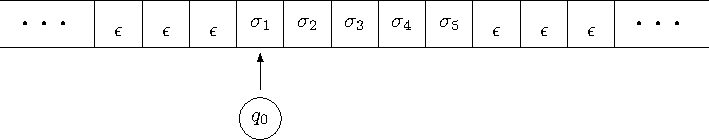
\includegraphics[scale=.7]{figures/tm-initial-input.pdf}
  \caption{Turing machine initialized with the input string $\sigma_1
    \sigma_2 \sigma_3 \sigma_4 \sigma_5$.}
\end{figure}
The ``program'' is then executed by the $\delta$ function. For
instance, suppose $\delta(q_0, \sigma_1) = (q_i, \gamma_1, R)$. Then
we interpret this as the Turing machine writing a $\gamma_1$ on the
current tape, updating its state to $q_1$, and moving one space to the
right on the tape.
\begin{figure}[H]
  \centering
  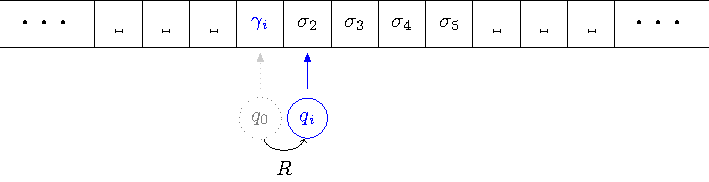
\includegraphics{figures/tm-one-step-later.pdf}
  \caption{Turing machine after performing a single step. Differences
    shown in {\color{blue} blue}.}
\end{figure}
At each step of the computation, the Turing machine performs a similar
process: Read the tape, rewrite and move as dictated by $\delta$, and
then repeat. If the Turing machine reaches the state $\cmark$, then it
halts and the input is said to be ``accepted.'' If it reaches
$\xmark$, the state is ``rejected.'' {\color{blue} In the case that
  the machine never halts, we treat this as a form of rejection.}




\section{Computational Universality}

A Universal Turing Machine is a Turing machine which can simulate any
arbitrary Turing Machine. It takes as its input a Turing Machine code $\langle M \rangle$ (for turing machine $M$ we'll denote the code of $M$ by $\langle M \rangle$), and an input word $w$, and then simulates what $M$ would do on input $w$. Intuitively, any modern computer is a (finite memory) Universal Turing Machine: it can store arbitrary computer programs as data, and then run them on other data it stores or with user input.

In a similar vein, a system is {\it computationally universal} (or
just {\it universal}) if it has the ability to simulate an arbitrary
Turing machine. This is a loose definition because it is not
immediately clear what it means for a dynamical system to simulate a
Turing machine. There are many possible ways to create a more precise
definition; we will follow the method of Delvenne et al. [CITATION].
Before we do, though, we note a few reasonable expectations about what
simulating a Turing machine should mean:

\begin{itemize}
  \item If a dynamical system can simulate an arbitrary Turing machine, we should be able to take any combination of Turing machine and input, and convert it into some question about the system. The question should be ``equivalent'' to the question of whether the Turing machine would accept its input, in the sense that it should have a ``yes'' answer if the Turing machine accepts, and a ``no'' answer if the Turing machine rejects or never halts.

  \item The Universal Turing Machine is a specific Turing Machine that exists, and therefore it is a dynamical system on the space of its possible configurations. We would definitely expect this dynamical system to be considered universal.

  \item There are a number of other computational models which have ability to simulate Turing Machines, and which can also be considered dynamical systems. One good example is cellular automata, which are like Turing machine tapes where every cell has its own state and updates itself based on its neighbors' states. If a given instance of a computation model is capable of simulating arbitrary Turing machines, we would expect its associated dynamical system to be universal.

\end{itemize}

\subsection*{Formally defining universality}

We will follow the lead of Delvenne et al. [CITATION] in defining what
it means for a dynamical system to be universal. Like them, we will
consider only {\it symbolic} dynamical systems, that is, dynamical
systems on spaces consisting of infinite words made out of symbols
drawn from a finite alphabet. We will need to do some spadework before
we're ready to give the full definition.

\subsubsection*{Spadework Part I - R.E.-completeness}

Our ultimate goal is, given the code for a Turing machine $M$, and the
input $w$, to ask a question about a particular dynamical system which
has a ``yes'' answer exactly when $M$ accepts $w$. In the terms used
in the field of computability, we want to be able to reduce an
arbitrary instance of the question ``Will Turing machine $M$ accept
the input $w$?'' to a question about the dynamical system.

Fortunately, much is already known about the question ``Will Turing
machine $M$ accept the input $w$?''. In particular, it is equivalent
to the question ``Will Turing machine $M$ halt on the input $w$?'' in
the sense that if we had a way to answer either of the questions, we
could easily answer the other as well. This second question is called
the Halting Problem, and computer scientists say that it is ``complete
for the class of recursively enumerable problems.''

So, depending on your background, you may be asking two questions:
``What is the class of recursively enumberable problems?'' and ``What
does it mean to be complete for it?'' A problem is called recursively
enumerable if it can be solved by a Turing machine that may not ever
halt, that is, if the question has a ``yes'' answer, the Turing
machine will accept in finite time, but if the question has a ``no''
answer, the machine may run indefinitely. They are called
``recursively enumerable'' because it would be possible for a Turing
machine (a computation model capable of {\it recursion}) to {\it
  enumerate} every input that would have a ``yes'' answer, in such a
way that every such input would eventually be listed in finite time.
(The machine could do this by listing all inputs lexicographically,
and spending half its time simulating the computation on the first
input, a quarter of its time on the second input, and so on, printing
out any input when it is accepted.)

A given problem, call it $P$, is complete for a class of problems,
$C$, if two conditions hold. First, $P$ must be an element of $C$.
Second, all problems in $C$ must be reducible to $P$, meaning that if
$P' \in C$, we can convert any instance of $P'$ to an instance of $P$
that will have the same answer, without doing an unreasonable amount
of work in the conversion (for our purposes here, any finite
computation time is reasonable). The Halting Problem is known to be
complete for the recursively enumerable problems, or r.e.-complete.

The question ``Will Turing machine $M$ accept input $w$?'' (call it
$Q$) is also r.e.-complete. Recall that our goal was to find a
question $QDS$ about a dynamical system, which we could reduce $Q$ to.
One way to express this constraint is that $QDS$ should be
r.e.-complete: then both $QDS$ and $Q$ could be reduced to each other,
so they would be equivalent questions, which is what we are looking
for. In fact, we will see that the r.e.-completeness of $QDS$ is
exactly what we will require.

\subsubsection*{Spadework Part II - Effective Symbolic Systems}

A symbolic set can be thought of as a set of words made from a finite alphabet $A$. We could express such a set as $(A \cup \{B\})^\Nn$, meaning the set of one-sided infinite words with characters which are either drawn from $A$ or are the ``blank'' symbol $B$. Finite words would then end be expressed as infinite words ending with an infinite tail of $B$s. But we could encode each element of $A \cup \{B\}$ with a binary sequence (with all encodings the same length), so any symbolic set can be encoded as a subset of the set $\{0,1\}^\Nn$ of one-sided infinite binary words.

We give $\{0,1\}^\Nn$ the following distance metric $d$: $d(x,y) = 0$ if $x$ and $y$ agree at all indices, and otherwise $d(x,y) = 2^{-n}$ where $n$ is the smallest index at which $x$ and $y$ differ. Under this metric, the set of all sequences beginning with a finite binary word $w$ is a both a closed and open set (a ``clopen'' set) under this metric. Call sets like this, generated by a common prefix, cylinders. It can be shown that the clopen sets of $\{0,1\}^\Nn$ are precisely the finite unions of cylinders. What is special about this is that we can associate with each clopen subset of $\{0,1\}^\Nn$ a unique finite set of finite words, which are the generating prefixes for the cylinders that make up that set. So we can express every clopen set of $\{0,1\}^\Nn$ in a finite way, which means the we can list off all the clopen sets in some lexicographic order (in other words, the set is countable). We'll be exploiting this fact later.

Now we're ready to define the main dynamical systems we'll be working with. If $X \subseteq \{0,1\}^\Nn$ is a symbolic set and $f: X \to X$ is a continuous map on $X$, then $(X, f)$ is an {\it effective symbolic system} if:
\begin{enumerate}[label=(\roman*)]
  \item $X$ is closed.
  \item Checking whether some clopen set $Y \subseteq \{0,1\}^\Nn$ has a non-zero intersection with $X$ is decidable by a Turing machine in finite time.
  \item The inverse map $f^{-1}$ on clopen sets of $X$ can be computed in finite time.
\end{enumerate}

These requirements may seem a bit arbitrary, but they are made for a good reason. We will shortly be performing some operations on the clopen sets of $X$, and it turns out that, since $X$ is closed, these are exactly the intersections of $X$ with the clopen sets of $\{0,1\}^\Nn$, so we know this is a countable set. Requirement (ii) helps ensure that a Turing machine could list out these clopen sets without ever getting stuck checking if a particular clopen set of $\{0,1\}^\Nn$ has a nonempty intersection with $X$. And requirement (iii) foreshadows operations we will be doing on clopen sets.

\subsubsection*{Spadework Part III - Temporal Logic}

Recall that we are looking for a way to ``ask questions'' about dynamical systems, whose answers will tell us something about the behavior of Turing machines. In order to be able to construct such questions, we will use subsets of state space to encode logical statements. Since we want to be able to make statements about the {\it eventual} behavior of the system, we will use a logical framework called temporal logic. Temporal logic includes all of the standard logical operators:
\begin{itemize}
  \item $\top$: always true
  \item $\bot$: always false
  \item $\lor$: or
  \item $\lnot$: not
  \item $\land$: and (which is actually redundant because it is constructible from $\lor$ and $\lnot$)
\end{itemize}
It adds two additional operators to the list:
\begin{itemize}
  \item $\lnext$: next, a unary operator, with $\lnext \phi$ meaning that $\phi$ will be true after one time step.
  \item $\ltil$: until, a binary operator, with $\phi \ltil \psi$ meaning that $\psi$ will be true within finite time, and for all time between the present and one step before the time when $\psi$ is true (inclusive), $\phi$ will be true
\end{itemize}

The developers of temporal logic, Arthur Prior and Hans Kamp, have described a set of rules for incorporating these operators into classical logic in a way that is consistent with our interpretation of them [CITATION]. For our purposes, suffice it to say that it works.

How do we propose to use temporal logic to construct statements about effective symbolic systems? Well, as we have suggested above, we are interested in operating on the clopen sets of symbolic systems, and here is where that will come into play. Let's say we have some effective dynamical system $(X, f)$. We will use the fact that the clopen subsets of $X$ are countable, and let $P_0, P_1, P_2, ...$ be a listing of all the clopen subsets of $X$ (including $\emptyset$ and $X$ in some positions).

Then let $\psc_0, \psc_1, \psc_2, ...$ be a set of propositional symbols, which are the logical ``units'' that along with the operators above are the building blocks of temporal logic formulas. The listing will contain $\top$ and $\bot$ in some positions. We're going to define an ``interpretation'' operator $\abs{\cdot}$ that takes logical formulas to subsets of $X$. The intuition behind it will be that if $\phi$ is a logical formula that expresses something about the ``current configuration of the system,'' $|\phi|$ is the set of possible system configurations (points of $X$) for which that statement is true. Formally, the operator will behave like this:

\begin{itemize}
  \item If $\phi$ is just the symbol $\psc_n$, $\abs{\phi} = P_n$, and we stipulate that the orderings should align such that $\abs{\top} = X$ and $\abs{\bot} = \emptyset$. This means that the symbol $\psc_n$ represents the statement ``The current system configuration is in the set $P_n$,'' which is of course always true if $P_n = X$ and never true if $P_n = \emptyset$.

  \item $\abs{\phi_1 \lor \phi_2} = \abs{\phi_1} \cup \abs{\phi_2}$, because for either $\phi_1$ or $\phi_2$ to be true, the system can be in any state in which either is true.

  \item $\abs{\lnot \phi} = X \setminus \abs{\phi}$, because the set of states for which $\phi$ is not true is the complement of the set of states for which it is.

  \item $\abs{\lnext \phi} = f^{-1}\left( \abs{\phi} \right)$, which means that $\lnext \phi$ represents the statement, $\phi$ will be true after one application of $f$, meaning that each application of $f$ corresponds to one ``time step'' within the temporal logic system. Note that we know that this is computable, by requirement (iii) of effective symbolic systems.

  \item $\abs{\phi_1 \ltil \phi_2} = \bigcup_{n \in \Nn} A_n$ with $A_0 = \abs{\phi_2}$ and the other sets defined by the recurrence relation $A_{n+1} = f^{-1}(A_n)\cap\abs{\phi_1}$. Here $A_n$ can be interpreted as, the set of system states for which $\phi_2$ will be true on the $n^{\text{th}}$ time step from the current state, and $\phi_1$ will be true on the $0,...n-1$ time steps. The union of all of these represents all states for which ``$\phi_1$ is true until $\phi_2$ is eventually true.''

    So, in short, we have used temporal logic to construct a set of formula that express statements about the state of the system. We say a given formula is satisfiable if its interpretation is non-empty, meaning that there is some nonempty set of $X$ that satisfies it.

\end{itemize}


\subsubsection*{Universality}

Our spadework concluded, we're ready to say what it means for an effective dynamical system to be universal. We will use Delvenne et. al's precise definition here:

``{\it An effective dynamical system is \emph{universal} if there is a recursive family of temporal formulae such that knowing whether a given formula of the family is satisfiable is an r.e.-complete problem.}''

A ``recursive'' family of temporal formulae is a set of temporal formula for which membership in the set can be decided by a turing machine in finite time; this is essentially a regularity condition which prevents the family from being outlandishly defined.

To get a feel for what this definition means, and ensure that it is reasonable, let's start by confirming that the Universal Turing Machine dynamical system  is, as we expected from the start, universal.

A configuration of the Universal Turing Machine, as with all Turing machines, is defined by finite control state and its tape contents, both of which can be encoded in a binary strings. So the configuration space of a UTM is a subset $X$ of $\{0,1\}^\Nn$, and the code for the UTM is some specific transition function on this space, $f$. Let's assume we are dealing with a a UTM that takes as input $\langle M \rangle, w, x$ with some special encoding of the delimiter ``$,$''. The machine first checks that its input is of this form, and halts immediately if it is not, and otherwise ignores $x$ and simulates $M$ on $w$. (We put the $x$ there so that we can have an arbitrary string on the end of our input, and the set of starting configurations given a specific choice of $M$ and $w$ will be a clopen set.)

To show this dynamical system is universal, we're looking for recursive family of formula whose satisfiability is r.e.-complete. Consider all the possible pairs of turing machine encodings, $\langle M \rangle$, and inputs $w$. Given such a pair, let $P_m$ represent the clopen set of all UTM configurations in the starting state and tape contents beginning with ``$\langle M \rangle , w,$''. Let $P_{h}$ represent the clopen set consisting of all halting configurations. (This will be clopen if we encode configurations in such a way that the finite control state is listed first, since the halt state will then be the common prefix). Then the formula corresponding to $M$ and $w$ is $$ \psc_{m} \land \Big( \top \ltil P_{h} \Big).$$ This formula's interpretation is the set of configurations which are in $P_m$ (they are starting configurations of the UTM which encode $M$ as the TM to simulate and $w$ as the input), and which will eventually halt. Since the UTM just does whatever $M$ would do on $w$, if the formula above is satisfiable, $M$ halts on $w$, and if it is not satisfiable, $M$ does not halt on $w$. So if we could answer the satisfiability question for all formulas of the form above, we would have a way to solve the halting problem. This means that the satisiability problem for this family of formulae is r.e.-complete, so the dynamical system is universal under the definition!

Similar arguments can be used to show that cellular automata and other models of computation capable of simulating Turing machines, when made into dynamical systems, satisfy our universality definition. What is interesting, though, is that this definition opens up the possibility that dynamical systems which are not immediately associated with Turing machines, might be universal. In fact, Delvenne et al. show that there does exist a system which is both chaotic and universal. They also show that certain properties of dynamical systems, like equicontinuity of the map, imply that a dynamical system cannot be universal.







\section{Appendix}
Here, we include some of the background definitions the reader might
not be acquainted with. First, we define a \emph{topology}.
\begin{definition}[Topology]
  Let $X$ be an arbitrary set. Let $\ms T$ be a collection of $U
  \subseteq X$ such that
  \begin{enumerate}
    \item (Containment of trivial elements): $\varnothing$, $X \in \ms
      T$,
    \item (Closure under arbitrary unions): For arbitrary collections
      $\set{U_i}_{i \in I} \subseteq \ms T$, we have
      \[
      \pn{\bigcup_{i \in I} U_i } \in \ms T,
      \]
      and
    \item (Closure under finite intersection): For finite collections
      $\set{U_i}_{i = 1}^n$, we have
      \[
      \pn{\bigcap_{i=1}^n U_i} \in \ms T. \qedhere
      \]
  \end{enumerate}
  Then we call $\ms T$ a \emph{topology} on $X$.
\end{definition}
The definition of a \emph{topology} is meant to axiomatize the
properties of \emph{open sets} that we encounter in analysis. Indeed,
one might note that in any metric space $X$, (1) both $\varnothing$
and $X$ are open sets, (2) open sets are closed under arbitrary union,
and (3) open sets are closed under finite intersection.

However, one should note that this is a \emph{proper} generalization,
in the sense that there exist topologies which cannot arise from a
metric. For instance, consider the following:
\begin{example}[Double-headed snake]
  Let $X = \set{0_{A}, 0_{B}} \cup \pb{0, 1}$. Here, the labels $A$
  and $B$ are just to distinguish the two ``copies'' of $0$ that we've
  made. Define a topology $\ms T$ on $X$ as follows:
  \begin{enumerate}
    \item Let $U \subseteq (0,1]$. Then if $U$ is open in $[0,1]$
      viewed as a metric space, we have $U \in \ms T$.
    \item Similarly: Given such a $U$, we have $\set{0_A} \cup U$,
      $\set{0_B} \cup U \in \ms T$. \qedhere
  \end{enumerate}
\end{example}
This effectively gives us a version of $[0,1]$ where we have two
copies of $0$. One can verify that the topology axioms are satisfied

So, why isn't this topology metrizable? In a nutshell, the problem is
that $0_A$, $0_B$ act as if they are distance $0$ apart from each
other, which breaks the ``$d(x,y) = 0 \iff x = y$'' axiom for metric
spaces.\footnote{A more rigorous argument can be constructed by noting
  that $\forall \varepsilon > 0$, $\set{0_A} \cup (0,\varepsilon)$ and
  $\set{0_B} \cup (0, \varepsilon)$ are open and then doing something
  like $0_A = \lim_{\varepsilon \to 0} \varepsilon = 0_B$, a
  contradiction.}

This underscores that topology is generally a more abstract way of
looking at properties of space. There are a number of situations in
which this abstraction is desired. First, it helps us to focus on
more ``abstract'' properties of space that are invariant under
stretching and deforming (but not gluing or tearing) --- e.g., in a
topological context, the two shapes shown in \cref{fig:deform-grid}
are the ``same.''
\end{multicols}
\begin{figure}[H]
  \centering
  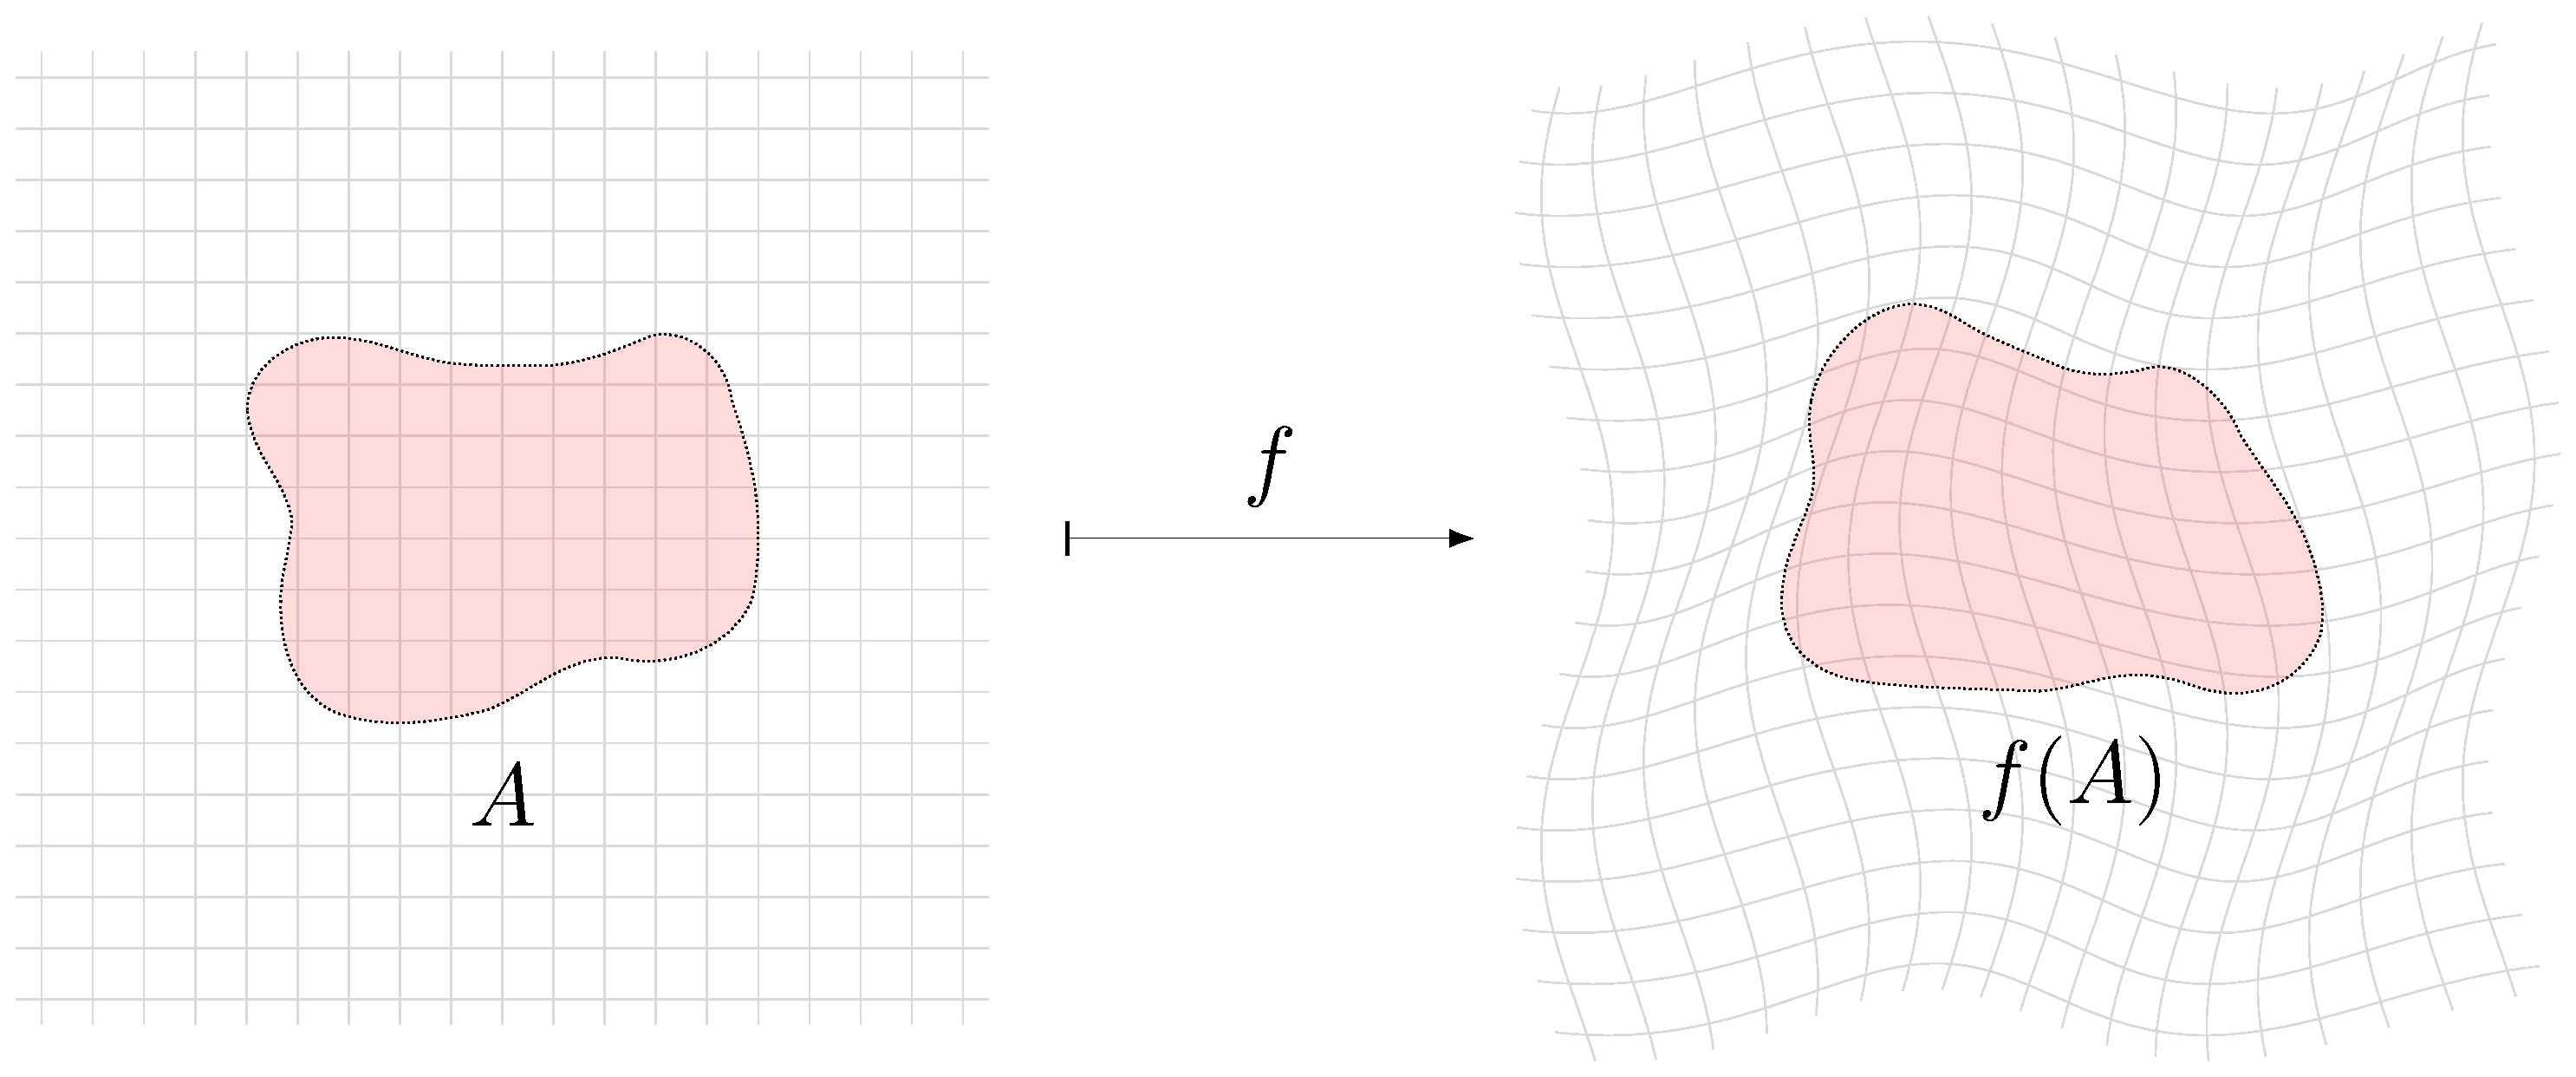
\includegraphics[scale=.325, angle=0]{figures/deform-grid.pdf}
  \caption{Two shapes that are topologically equivalent}
  \label{fig:deform-grid}
\end{figure}
\begin{figure}[H]
  \centering
  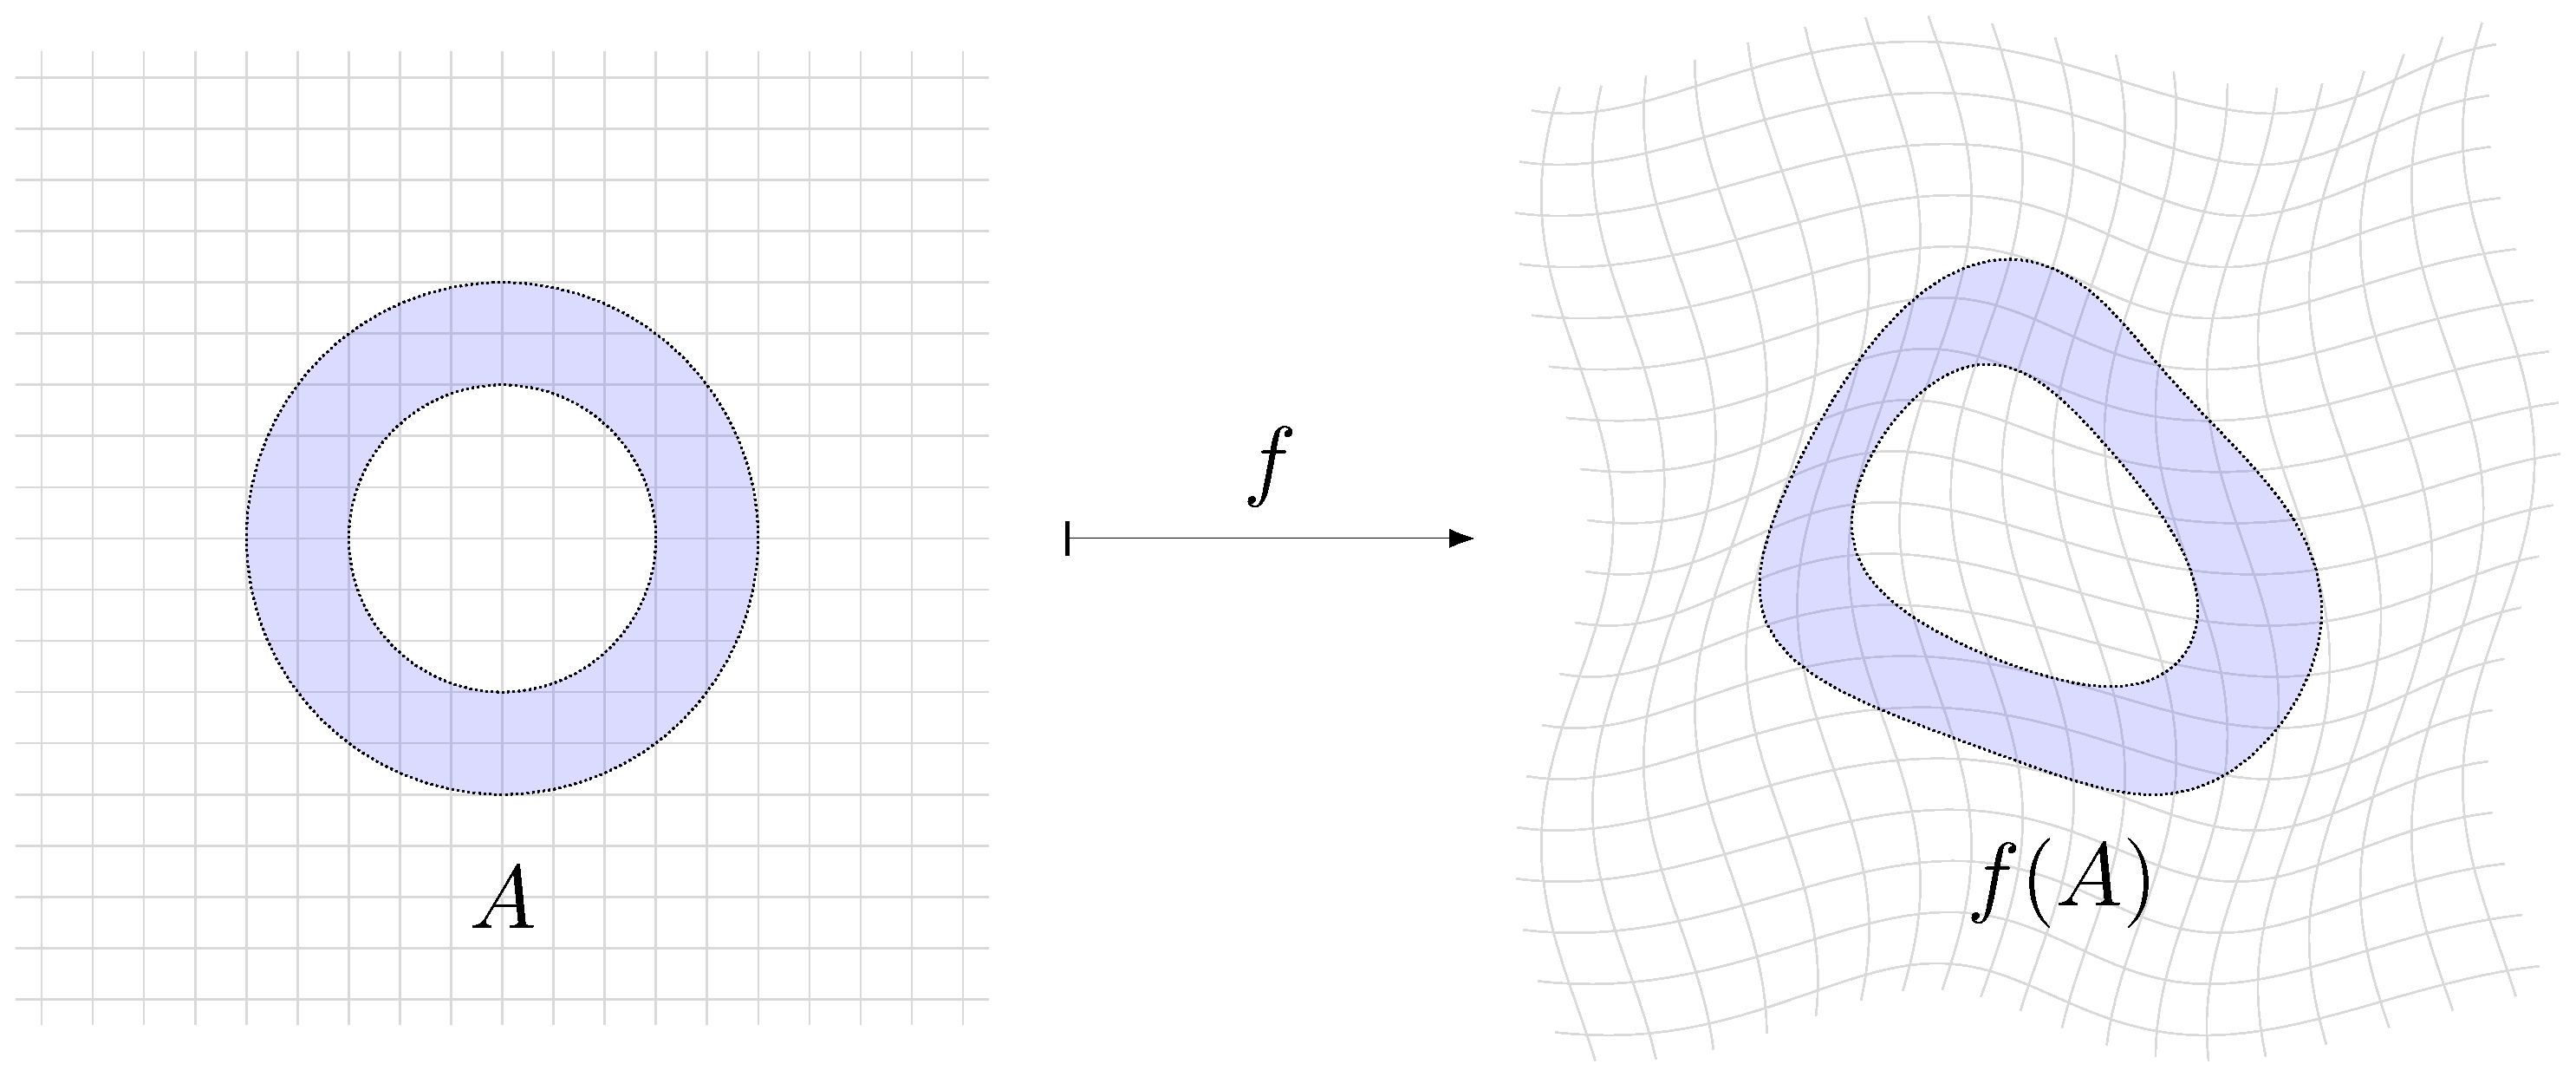
\includegraphics[scale=.325, angle=0]{figures/deform-grid-annulus.pdf}
  \caption{Two shapes that are topologically equivalent to each other,
    but not to those in \cref{fig:deform-grid}}
  \label{fig:deform-annulus}
\end{figure}
\begin{multicols}{2}
  Often, these are the kinds of properties we're interested in when we
  try to find ways of thinking of {\color{red} random sets $X$ that
    we've just scooped out of a bush on the side of the street in
    terms of ``spaces.''} Understanding exactly what we mean by
  invariance under ``stretching and deforming'' is the subject of the
  next section.

  % {\color{blue} is there more to say here?}

  \subsection{Continuity}
  In abstract algebra, we define \emph{homomorphisms} to be functions
  that preserve the ``structure'' of algebraic objects like groups,
  rings, and so on. In linear algebra, \emph{linear transformations}
  similarly preserve the structure of vector spaces.
  \emph{Isomorphisms} in group theory provide a sense of ``perfect,
  reversible matching,'' just as \emph{invertible linear
    transformations} (``vector space isomorphisms'') do in linear
  algebra.

  These are examples of \emph{morphisms}, a broader term for
  structure-preserving maps {\color{red} that sees a lot of tasteless
    name-dropping by people like us who got too excited about category
    theory once upon a time.} In defining an abstract topology, we
  have created a structure. We now define the maps that preserve that
  structure. The answer is continuous functions, and the inspiration
  comes from thinking about continuous functions in metric spaces.

  Let $(E,d)$, $(E', d')$ be metric spaces, and let $f : E \to E'$ be
  continuous. Then recall the following properties of $f$:
  \begin{itemize}
    \item For all compact sets $V \subseteq E$, $f(V)$ is compact in
      $E'$,
    \item For all connected sets $C \subseteq E$, $f(C)$ is connected
      in $E'$, and
    \item For all open sets $U \subseteq E'$, the inverse image
      $f^{-1}(U)$ is open in $E$. In fact, this is an equivalent way
      to characterize continuity.
  \end{itemize}
  For all these reasons (especially the final one), it turns out that
  continuous functions provide the natural definition of morphism for
  our topological spaces. We can loosely interpret continuous
  functions as preserving the notion of \emph{closeness} of points,
  which is essentially the fundamental ``structure'' of a metric
  space. Again, this is analogous to the definition of a group
  homomorphism
  \[
    \varphi({\color{blue}g} + {\color{blue}h}) = \varphi({\color{blue}
      g}) + \varphi({\color{blue} h}),
  \]
  or a linear transformation
  \[
    T({\color{orange} c_1} {\color{blue}u} + {\color{orange} c_2}
    {\color{blue} v})) = {\color{orange} c_1} T({\color{blue} u}) +
    {\color{orange} c_2} T({\color{blue} v}).
  \]
  In particular, writing out the definition of continuity, we see that
  it has the same basic structure of ``property in the domain is
  preserved in the codomain:''
  \[
    d({\color{blue} x_0, x_1}) < \delta \implies
    d(f({\color{blue}x_0}), f({\color{blue}x_1})) < \varepsilon.
  \]
  The details get slippery if you poke around too closely, but the
  intuition is there. Anyways: Since not all topologies are
  metrizable, we choose a definition that relies only on topological
  structure, but which coincides with continuity in the case of metric
  spaces.
  \begin{definition}[Continuous function]
    Let $(X, \ms T_X)$, $(Y, \ms T_Y)$ be topological spaces. Let $f :
    X \to Y$. Then we say $f$ is \emph{continuous} iff for all $U\in
    \ms T_Y$,
    \[
      f^{-1}(U) \in \ms T_X. \qedhere
    \]
  \end{definition}
  This is a bit strange, since the structure-preservation occurs in
  taking the inverse image, not the image. We won't go into the weeds
  of trying to interpret this, and will instead just talk about the
  concept that \emph{does} port well: topological isomorphism, almost
  universally referred to as \emph{homeomorphism}.
  \begin{definition}[Homeomorphism]
    Let $(X, \ms T_X)$, $(Y, \ms T_Y)$ be topological spaces. Let $f :
    X \to Y$ be continuous and bijective. Further suppose $f^{-1}$ is
    continuous. Then we call $f$ a \emph{homeomorphism}.
  \end{definition}
  Homeomorphisms provide the rigorous underpinning for thinking about
  ``smooth deformations'' on a space.

  {\color{blue} insert some discussion of bases in linear algebra and
    generators in abstract algebra and how a base is kinda like that}

  {\color{blue} also insert some discussion of manifolds}


  \begin{definition}[Base]\label{def:base}
    Let $(X, \ms T)$ be a topological space. Let $\ms B \subseteq \ms
    T$ such that
    \begin{enumerate}
      \item (Covering): We have
        \[
        \bigcup_{B \in \ms B} B = X,
        \]
        and
      \item (Intersection stuff): For all $B_1, B_2 \in \ms B$ and
        for all $x \in B_1 \cap B_2$, there exists $B_3 \in \ms B$
        such that $x \in B_3$ and
        \[
        B_3 \subseteq B_1 \cap B_2.
        \]
      \item (Generation by union): For all $U \in \ms T$, there exists
        $\ms B' \subseteq \ms B$ such that
        \[
        \bigcup_{B \in \ms B'} B = U.
        \]
    \end{enumerate}
    Then we call $\ms B$ a \emph{base} or \emph{basis} for the
    topology $\ms T$.
  \end{definition}
  These properties should be reminiscent of open balls in $\RR^n$.
  Note that open balls (1) cover $\RR^n$, and (2) satisfy the
  ``intersection stuff'' property --- namely, although the
  intersection of two open balls $B_1, B_2$ is generally not another
  open ball, for each $x \in B_1 \cap B_2$, we can find a \emph{third}
  open ball $B_3$ such that $x \in B_3 \subseteq B_1 \cap B_2$. A base
  is meant to extend this idea to general topologies.


\end{multicols}







\end{document}
